\documentclass[11pt]{article}

\newcommand{\cnum}{CS188}
\newcommand{\ced}{Winter 2017}
\newcommand{\ctitle}[3]{\title{\vspace{-0.5in}\cnum, \ced\\Problem Set #1: #2\\Due #3}}
\usepackage{enumitem}
\usepackage{mathtools}
\usepackage{amsmath}

\usepackage{graphicx}
\newcommand{\solution}[1]{{{\color{blue}{\bf Solution:} {#1}}}}
\usepackage[usenames,dvipsnames,svgnames,table,hyperref]{xcolor}

\renewcommand*{\theenumi}{\alph{enumi}}
\renewcommand*\labelenumi{(\theenumi)}
\renewcommand*{\theenumii}{\roman{enumii}}
\renewcommand*\labelenumii{\theenumii.}


\begin{document}
\ctitle{3}{SVM and Kernels}{March 2,2017}
\author{}
\date{}
\maketitle
\vspace{-0.75in}

\section{Problem 1}
\begin{enumerate}
\item Problem 1a

\solution{
Yes, the function is a kernel. We can show that $k(x, z)$ is a kernel by considering an arbitrary $2 x 2$ kernel matrix $K$ that defines the quantities $k(x, x)$, $k(x, z)$, $k(z, x)$, $k(z, z)$. In particular, let $k(x, x) = a$, which is simply the number of unique elements in the document x, and similarly let $k(z, z) = c$. Also, let the unique words in the intersection of documents x and z be given by $k(z, x) = k(x, z) = b$. We note that $k(z, x) = k(x, z)$ since set intersection is commutative. Then, \[ K = \begin{bmatrix} k(x,x) =a & k(x,z) =b \\ k(z,x)=b & k(z,z)=c \end{bmatrix} \] . 

Importantly, $a \geq b$ and $c \geq b$, since the size of the intersection of two sets can never exceed the size of a set intersected with itself. 

To show that $k(x,z)$ is a kernel, we must show this matrix is PSD, or all its eigenvalues $\lambda \geq 0 $. 

\[det(K - \lambda I) = (a - \lambda)(c - \lambda) -b^2 = 0 \]. 

Solving for $\lambda$, 
\[ \lambda_1 = \frac{a + c -\sqrt{(a-c)^2 + 4b^2}}{2} \]
\[ \lambda_2 = \frac{a + c + \sqrt{(a-c)^2 + 4b^2}}{2} \]

$\lambda_2$ is clearly $\geq 0$, and we want to see if $\lambda_1$ is also: 

\[ \lambda_1 \geq 0 \rightarrow{} \frac{a + c - \sqrt{(a-c)^2 + 4b^2}}{2} \geq 0\]
\[(a+c)^2 \geq (a-c)^2 + 4b^2 \]
\[4ac \geq 4b^2 \rightarrow{} ac \geq b^2 \] which is true since we established earlier that $a \geq b$ and $c \geq b$. 
We have shown that all eigenvalues are non-negative, so the kernel matrix is PSD, and therefore $k(x,z)$ is a kernel. 

}

\vspace{1cm}
\item Problem 1b

\solution{
We have to show that $(1 + (\frac{x}{||x||)} (\frac{z}{||z||}))^3$ is a kernel. \newline{}

$x \cdot z$ is a kernel, so by the scaling rule where we let $f(x) = \frac{1}{||x||}$ and $f(z) = \frac{1}{||z||}$, we see that $\frac{x \cdot z}{||x||||z||}$ is also a kernel. \newline{}

Next, $k(x,z) = 1$ is also a kernel since the associated kernel matrix $K \in R^{N xN}$ consists of all 1s, so this matrix has $N$ eigenvalues that are $\geq 0$, one of which is $N$ and the others is $0$ with algebraic multiplicity $N-1$. \newline{}

So since $k(x,z) = 1$ and $\frac{x \cdot z}{||x||||z||}$ are both kernels, the sum is also a kernel by the sum rule. \newline{}

Now we have a function $ f(x,z) = (1 + (\frac{x}{||x||)} (\frac{z}{||z||}))^3$. \newline{}

The quantity inside has been shown to be a kernel, so we can apply the product rule since we are multiplying a kernel with itself 3 times (To be completely precise, we apply the product rule twice, first to show that $(1 + (\frac{x}{||x||)} (\frac{z}{||z||}))^2$ is a kernel and then once again to get the final result). \newline{}

Therefore, the given quantity is indeed a kernel.
}
\vspace{1cm}
\item Problem 1c

\solution{
We have $K_{\beta} = (1 + \beta x \cdot z)^3 = (1 + \beta(x_1z_1 + x_2z_2))^3$ \newline{}

Using WolframAlpha to expand this, we obtain the expression for $K_\beta$ 
\[ K_\beta = 1 + 3 \beta x_1z_1 + 3\beta x_2z_2 + 3 \beta^2 x_1^2z_1^2 + 6\beta^2 x_1 x_2 z_1 z_2 + \] $3\beta^2 x_2^2 z_2^2 + \beta^3 x_1^3 z_1^3 + 3\beta^3 x_1^2 x_2 z_1^2 z_2 + 3\beta^3 x_1 x_2^2 z_1 z_2^2 + \beta^3 x_2^3 z_2^3 $ \newline{}

Since we kernels to replace inner products between transformed feature vectors, this expression is equal to $\phi(x)^T \phi(z)$ for some $\phi$ that we need to determine. \newline{}

By inspection, we determine that \[ \phi(x) = \begin{bmatrix} 1 \\ \sqrt{3}x_1 \beta^{\frac{1}{2}} \\ \sqrt{3}x_2 \beta^{\frac{1}{2}} \\ \sqrt{3} x_1^2 \beta \\ \sqrt{6}x_1 x_2 \beta \\ \sqrt{3} x_2^2 \beta \\x_1^3 \beta^{\frac{3}{2}} \\ \sqrt{3}x_1^2 x_2 \beta^{\frac{3}{2}} \\ \sqrt{3}x_1 x_2^{2} \beta^{\frac{3}{2}} \\ x_2^3 \beta^{\frac{3}{2}} \end{bmatrix} \] If we take the corresponding $\phi(z)$ and compute the inner product, we end up with the expression for $K_{\beta}$. \newline{}

Comparing to the kernel $k(x,z) = (1 + x \cdot z)^3 $ we see that the feature transformation functions are similar, the only difference is that the $\phi$ corresponding to $k(x,z) = (1 + x \cdot z)^3 $ is not multiplied by a constant $\beta$ to some power in every element. Besides that, they have the same arrangement of pairwise combinations of the features. \newline{}

The role of the parameter $\beta$ appears to be to scale each element of the feature vector by a constant raised to a certain power. For smaller combinations of features, such as just $x_1 x_2$, the scaling is just done by a factor of $\beta$, but for larger combinations, it's done by $\beta^{\frac{3}{2}}$. If $ 0 < \beta < 1$, then if we have very large combinations, the associated parameter $\beta$ will be raised to a higher power, causing that specific (transformed) feature to be very small and have less of an impact on the learning model. 
}
\end{enumerate}

\newpage
\section{Problem 2}

\item Problem 2a
\solution{
We have $min_\theta \frac{1}{2} || \theta ||^2 $s.t.  $y_1 \theta^T x_1 \geq 1$ \newline{}
Since $y_n = -1$ and $x = (a,e)^T$, we have $min_\theta \frac{1}{2} || \theta ||^2 $s.t.$ - \theta (a,e)^T \geq 1$ \newline{}

The primal can be written as: \[ p* = min_{\theta} max_{\alpha} L(\theta, \alpha) \] where \[ L(\theta, \alpha) = \frac{1}{2} ||\theta||^2 + \alpha( \theta (a,e)^T + 1) \] the dual is \[ d* = max_\alpha g(\alpha) \] where \[ g(\alpha) = min_{\theta} L(\theta, \alpha) \] differentiating $L$ with respect to $\theta$ first, we get \[ \frac{\delta L}{\delta \theta} = 0 \rightarrow{} \theta + \alpha x^T =0 \rightarrow{} \theta = -\alpha x^T \] \[ \theta = -\alpha (a,e)^T \] We now maximize over $\alpha$: \[ max_\alpha \frac{1}{2} || -\alpha (a,e)^T || + \alpha( -\alpha(a,e)^T(a,e) + 1) \] \[ max_\alpha \frac{1}{2}(\alpha^2 a^2 + \alpha^2 e^2) + \alpha(-\alpha a^2 -\alpha e^2 + 1) \] \[ max_\alpha \frac{-\alpha^2(a^2 + e^2)}{2} + \alpha \] \[ \frac{\delta}{\delta \alpha} = 0 \rightarrow{} -\alpha(a^2 + e^2) + 1 =0 \rightarrow{} \alpha = \frac{1}{a^2 + e^2} \] Substituting back into the expression for $\theta*$, we obtain \[ \theta* = -\frac{1}{a^2 + e^2} \begin{bmatrix} a \\ e \end{bmatrix} \]
}
\item Problem 2b
\solution{
We want \[ min_\theta \frac{1}{2} || \theta||^2 \] s.t. \[(1)(\theta_1 + \theta_2) \geq 1 \] and \[ (-1)(\theta_1) \leq 1\]
The lagrangian is \[ L(\theta, \alpha) = \frac{1}{2}(\theta_1^2 + \theta_2^2) + \alpha_1(1 - \theta_1 -\theta_2) + \alpha_2(1 + \theta) \] The dual problem is given by \[ d* = max_\alpha min_\theta L(\theta, \alpha) \] We first minimize with respect to $\theta$: \[ \frac{\delta L}{\delta \theta_1} = \theta_1 -\alpha_1 + \alpha_2 = 0 \rightarrow{} \theta_1 = \alpha_1 - \alpha_2 \]
\[ \frac{\delta l}{\delta \theta_2} = \theta_2 - \alpha  = 0 \rightarrow{} \theta_2 = \alpha_1 \] 
Now, $g(\alpha)$ can be given by \[ g(\alpha) = \frac{1}{2} (\alpha_1^2 -2\alpha_1 \alpha_2 + \alpha_2^2 + \alpha_1^2) + \alpha_1(1 - 2\alpha_1 + \alpha_2) + \alpha_2(\alpha_1 - \alpha_2 + 1) \]
\[ \frac{\delta g}{\delta \alpha_1} = -2\alpha_1 + \alpha_2 + 1 = 0 \rightarrow{} \alpha_1 = \frac{\alpha_2 + 1}{2} \]
\[ \frac{\delta g}{\delta \alpha_2} = -\alpha_2 + 1 + \alpha_1 \rightarrow{} \alpha_2  = \alpha_1 + 1 \]
\[ \alpha_1 = 2, \alpha_2 = 3 \]
Plugging back into $\theta$, this gives us \[ \theta_1 = -1, \theta_2 = 2, \theta* = \begin{bmatrix} -1 \\ 2 \end{bmatrix} \]
The margin is $\gamma = \frac{1}{||\theta||_2^2} = \frac{1}{\sqrt{5}} $
}

\item Problem 2c

\solution{
We now have the problem \[ min_\theta \frac{1}{2} ||\theta||_2^2 \] such that \[ \theta_1 + \theta_2 + b \geq 1\] and \[ -1(\theta_1 + b) \geq 1\]
The lagrangian is \[ L(\theta, b, \alpha) = \frac{1}{2}[\theta_1^2 + \theta_2^2] + \alpha_1( (1-b) -\theta_1 -\theta_2) + \alpha_2 ( (1 + b) + \theta_1_) \]

Solving for $\theta$, we obtain: 
\[ \frac{\delta L}{\delta \theta_1} = \theta_1 - \alpha_1 + \alpha_2 \rightarrow{} \theta_1 = \alpha_ 1 - \alpha_2 \]
\[ \frac{\delta L}{\delta \theta_2} = \theta_2 - \alpha_1 = 0 \rightarrow{} \theta_2 = \alpha_1 \]
We then obtain $g(\alpha, b)$ as \[ g(\alpha, b) = -\alpha_1^2 - \frac{1}{2}\alpha_2^2 + \alpha_1 \alpha_2 + \alpha_1(1-b) + \alpha_2(1 + b) \]
\[\frac{\delta g}{\delta a_1} = -2\alpha_1 + \alpha_2 + 1 - b = 0 \rightarrow{} \alpha_1 = \frac{\alpha_2 + 1 -b}{2} \]
\[\frac{\delta g}{\delta a_2} = -\alpha_2 + \alpha_1 + 1 + b = - \rightarrow{} \alpha_2 = \alpha_1 + 1 + b \]
\[ \frac{\delta g}{\delta b} = b(\alpha_2 - \alpha_1) = 0 \]
Case 1: $b = 0$ gives us $\theta*$ the same as in part 2B, the previous problem. 
Case 2: $ \alpha_1 - \alpha_2 = 0 $: \[ \alpha_2 = \alpha_1 \] \[ \alpha_1 = \frac{\alpha_1 + 1 -b}{2} \] \[ \alpha_1 = 1 - b \] \[ \alpha_1 = \alpha_1 + 1 + b \] \[b = -1, \alpha_1 = \alpha_2 = 2 \] \[ \theta_1 = \alpha_1 - \alpha_2 = 0, \theta_2 = \alpha_2 = 2 \]
\[ \theta* = \begin{bmatrix} 0 \\ 2 \end{bmatrix}, b* = -1, \gamma = \frac{1}{2} \]
Without offset, we had \[ \theta* = \begin{bmatrix} 1 \\ -2 \end{bmatrix}, \gamma = \frac{1}{\sqrt{5}} \]
By having an offset bias term, we ended up with a larger margin for our decision boundary.
}
\newpage

\section{Problem 3}
\item Problem 3.2b
\solution{
It might be beneficial to maintain class proportions across folds because if we had an imbalance of classes, our classifier will not have enough training examples to learn the decision boundary that separates the classes very well. In the extreme case, if our classifier trained on a fold with no negative examples at all, it would not learn that negative examples even exist and hence would produce a decision boundary that fails to generalize at all. If the class proportions were perfectly balanced, then our classifier will not be biased to fitting a hyperplane that "prefers" one class over the other. 
}
\item Problem 3.2d \newline{}
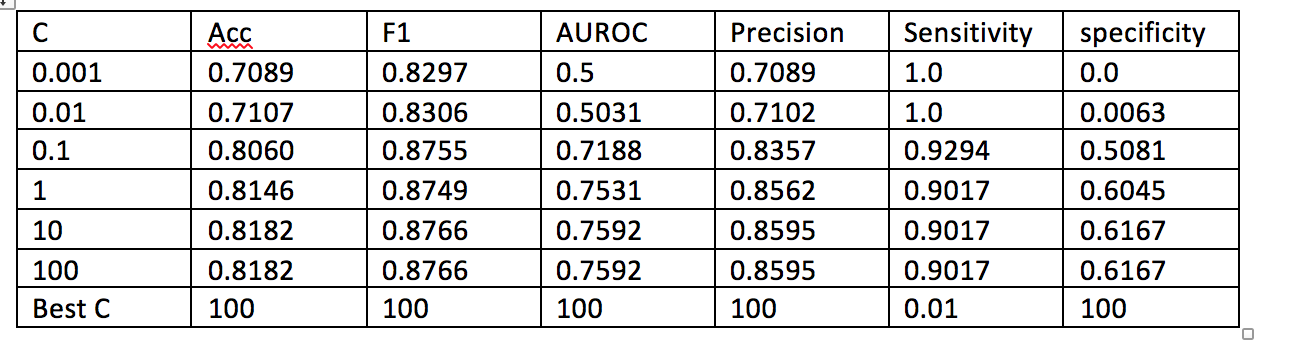
\includegraphics[scale=0.75]{t1.png}
\newline{}
In general, the performance tends to increase as C increases, but stays roughly the same for larger C (like 100 or 10). However, for sensitivity, the performance actually decreasers as C increases, and is roughly the same for C = 1, 10, 100. For speciificty, the performance is nearly C for the smallest C, and then begins to increase and plateu around 0.6 as C increases. With respect to the performance metric, the main one that deviates from the general trend is sensitivity. It seems that with respect to the sensitivity accuracy, we have overfit on the data because when C is small, the slack variablses are not penalized at all. Since we're allowed to have slack variables, all of the labels are memorized and we don't generalize. 
\item Problem 3.3a
\solution{
Consider $k(x_i, x_j)$ being the rbf kernel. A small gamma means that the influence of $x_j$ in the kernel is more, in other words, if $x_j$ is a support vector, a small gamma means that the support vector will have a large influence on deciding the class of the other training example $x_i$. If the gamma is large, then the variance is small (and the bias is high), meaning that the support vector won't have much influence on the label of the training example $x_i$. Large gamma = high bias and low variance model, and small gamma = low bias and high variance. 
}
\item Porblem 3.3b
\solution{
The grid I used were all the pairwise combinations C = [0.001, 0.01, 0.1, 1, 10, 100] and $\gamma=$ [0.001, 0.01, 0.1, 1, 10, 100]. The reason I chose this grid was because it used all of the C values that we used in our linear kernel, and I picked the same gamma because it covered a wide range, from very small values of gamma to very large gamma. Therefore, my grid considered all the pairings of small and large gamma, giving us a wide variety of hyperparameter settings. 
}

\item Problem 3.3c
\solution{ Here, g = the gamma value that was found. \newline{}
Acc: C = 100, g = 0.01, score = 0.8165

F1 score: C = 100, g = 0.01, score = 0.8763

Auroc: C = 100, g = 0.01, score = 0.7545

Precision: C = 100, g = 0.01, score = 0.8583

Sensitivity: C = 0.1, g = 100, score = 1.0 (several other combinations have a score of 1.0 also, such as C = 0.01, 10) being an example)

Specificity: C = 100, g = 0.01, score = 0.6047

\newline{}

\newline{}

The CV peformance is similar to the linear kernel, the most common best pair that we obtained was C = 100, g = 0.01. In particular, a large value of C that penalizes slack variables well, and a small gamma, that indicates a lower bias, higher variance (relative to other values of gamma) model worked well. We had metrics around 0.7 and 0.8 for most of the classes, and once again sensitivity was a bad metric for gauging our model, because the sensitivity metric rewards classifiers that just memorize the data. Only the sensitivity metric gave us the best C = 0.1 and g = 100, because the sensitivity metric let us overfit so we did not penalize slack variables very much and our high gamma indicates a model with high bias and low variance, another inidication of overfitting. 
}
\item Problem 3.4a
\solution{
For the linear SVM, I used C = 100 because this was the most common best C that we obtained (C = 100 showed up 5 out of 6 times in problem 3.2b). For the rbf kernel, I used C = 100, g = 0.01 because once ogain this was the most common best pair that we obtained. 
}
\newpage
\item problem 3.4c

\solution{
\newline{}

Metric: accuracy, linear score: 0.742857142857 ,rbf score: 0.757142857143

Metric: f1score, linear score: 0.4375 ,rbf score: 0.451612903226

Metric: auroc, linear score: 0.625850340136 ,rbf score: 0.636054421769

Metric: precision, linear score: 0.636363636364 ,rbf score: 0.7

Metric: sensitivity, linear score: 0.333333333333 ,rbf score: 0.333333333333

Metric: specificity, linear score: 0.918367346939 ,rbf score: 0.938775510204

For the accuracy, f1, auroc, sensitivity, and specifity metrics, the linear and rbf kernel svms did about the same, with the rbf kernel beating out the linear kernel slightly. We note that our hypothesis of the sensitivity being a metric that is prone to overfitting turned out to be true, since we had the poorest generalization, indicated by the lowest score, on an unseen test data set. Overall, the metric that corresponds to the highest csore is the sepecifify. Our gaussian rbf kernel beats out our linear kernel slightly in all of the metrics, the largest differences being in the precision metric. 
}
\end{document}
